\documentclass[a4paper]{article}
\usepackage[a4paper, margin=1in]{geometry}
% Some basic packages
\usepackage[utf8]{inputenc}
\usepackage[T1]{fontenc}
\usepackage{textcomp}
\usepackage[dutch]{babel}
\usepackage{url}
\usepackage{graphicx}
\usepackage{float}
\usepackage{booktabs}
\usepackage{enumitem}

\pdfminorversion=7

% Don't indent paragraphs, leave some space between them
\usepackage{parskip}

% Hide page number when page is empty
\usepackage{emptypage}
\usepackage{subcaption}
\usepackage{multicol}
\usepackage{xcolor}

% Other font I sometimes use.
% \usepackage{cmbright}

% Math stuff
\usepackage{amsmath, amsfonts, mathtools, amsthm, amssymb}
% Fancy script capitals
\usepackage{mathrsfs}
\usepackage{cancel}
% Bold math
\usepackage{bm}
% Some shortcuts
\newcommand\N{\ensuremath{\mathbb{N}}}
\newcommand\R{\ensuremath{\mathbb{R}}}
\newcommand\Z{\ensuremath{\mathbb{Z}}}
\renewcommand\O{\ensuremath{\emptyset}}
\newcommand\Q{\ensuremath{\mathbb{Q}}}
\newcommand\C{\ensuremath{\mathbb{C}}}

% Easily typeset systems of equations (French package)
\usepackage{systeme}

% Put x \to \infty below \lim
\let\svlim\lim\def\lim{\svlim\limits}

%Make implies and impliedby shorter
\let\implies\Rightarrow
\let\impliedby\Leftarrow
\let\iff\Leftrightarrow
\let\epsilon\varepsilon

% Add \contra symbol to denote contradiction
\usepackage{stmaryrd} % for \lightning
\newcommand\contra{\scalebox{1.5}{$\lightning$}}

% \let\phi\varphi

% Command for short corrections
% Usage: 1+1=\correct{3}{2}

\definecolor{correct}{HTML}{009900}
\newcommand\correct[2]{\ensuremath{\:}{\color{red}{#1}}\ensuremath{\to }{\color{correct}{#2}}\ensuremath{\:}}
\newcommand\green[1]{{\color{correct}{#1}}}

% horizontal rule
\newcommand\hr{
    \noindent\rule[0.5ex]{\linewidth}{0.5pt}
}

% hide parts
\newcommand\hide[1]{}

% si unitx
\usepackage{siunitx}
\sisetup{locale = FR}

% Environments
\makeatother
% For box around Definition, Theorem, \ldots
\usepackage{mdframed}
\mdfsetup{skipabove=1em,skipbelow=0em}
\theoremstyle{definition}
\newmdtheoremenv[nobreak=true]{definitie}{Definitie}
\newmdtheoremenv[nobreak=true]{eigenschap}{Eigenschap}
\newmdtheoremenv[nobreak=true]{gevolg}{Gevolg}
\newmdtheoremenv[nobreak=true]{lemma}{Lemma}
\newmdtheoremenv[nobreak=true]{propositie}{Propositie}
\newmdtheoremenv[nobreak=true]{stelling}{Stelling}
\newmdtheoremenv[nobreak=true]{wet}{Wet}
\newmdtheoremenv[nobreak=true]{postulaat}{Postulaat}
\newmdtheoremenv{conclusie}{Conclusie}
\newmdtheoremenv{toemaatje}{Toemaatje}
\newmdtheoremenv{vermoeden}{Vermoeden}
\newtheorem*{herhaling}{Herhaling}
\newtheorem*{intermezzo}{Intermezzo}
\newtheorem*{notatie}{Notatie}
\newtheorem*{observatie}{Observatie}
\newtheorem*{oef}{Oefening}
\newtheorem*{opmerking}{Opmerking}
\newtheorem*{praktisch}{Praktisch}
\newtheorem*{probleem}{Probleem}
\newtheorem*{terminologie}{Terminologie}
\newtheorem*{toepassing}{Toepassing}
\newtheorem*{uovt}{UOVT}
\newtheorem*{vb}{Voorbeeld}
\newtheorem*{vraag}{Vraag}

\newmdtheoremenv[nobreak=true]{definition}{Definition}
\newtheorem*{eg}{Example}
\newtheorem*{notation}{Notation}
\newtheorem*{previouslyseen}{As previously seen}
\newtheorem*{remark}{Remark}
\newtheorem*{note}{Note}
\newtheorem*{problem}{Problem}
\newtheorem*{observe}{Observe}
\newtheorem*{property}{Property}
\newtheorem*{intuition}{Intuition}
\newmdtheoremenv[nobreak=true]{prop}{Proposition}
\newmdtheoremenv[nobreak=true]{theorem}{Theorem}
\newmdtheoremenv[nobreak=true]{corollary}{Corollary}

% End example and intermezzo environments with a small diamond (just like proof
% environments end with a small square)
\usepackage{etoolbox}
\AtEndEnvironment{vb}{\null\hfill$\diamond$}%
\AtEndEnvironment{intermezzo}{\null\hfill$\diamond$}%
% \AtEndEnvironment{opmerking}{\null\hfill$\diamond$}%

% Fix some spacing
% http://tex.stackexchange.com/questions/22119/how-can-i-change-the-spacing-before-theorems-with-amsthm
\makeatletter
\def\thm@space@setup{%
  \thm@preskip=\parskip \thm@postskip=0pt
}


% Exercise 
% Usage:
% \oefening{5}
% \suboefening{1}
% \suboefening{2}
% \suboefening{3}
% gives
% Oefening 5
%   Oefening 5.1
%   Oefening 5.2
%   Oefening 5.3
\newcommand{\oefening}[1]{%
    \def\@oefening{#1}%
    \subsection*{Oefening #1}
}

\newcommand{\suboefening}[1]{%
    \subsubsection*{Oefening \@oefening.#1}
}


% \lecture starts a new lecture (les in dutch)
%
% Usage:
% \lecture{1}{di 12 feb 2019 16:00}{Inleiding}
%
% This adds a section heading with the number / title of the lecture and a
% margin paragraph with the date.

% I use \dateparts here to hide the year (2019). This way, I can easily parse
% the date of each lecture unambiguously while still having a human-friendly
% short format printed to the pdf.

\usepackage{xifthen}
\def\testdateparts#1{\dateparts#1\relax}
\def\dateparts#1 #2 #3 #4 #5\relax{
    \marginpar{\small\textsf{\mbox{#1 #2 #3 #5}}}
}

\def\@lecture{}%
\newcommand{\lecture}[3]{
    \ifthenelse{\isempty{#3}}{%
        \def\@lecture{Lecture #1}%
    }{%
        \def\@lecture{Lecture #1: #3}%
    }%
    \subsection*{\@lecture}
    \marginpar{\small\textsf{\mbox{#2}}}
}



% These are the fancy headers
\usepackage{fancyhdr}
\pagestyle{fancy}

% LE: left even
% RO: right odd
% CE, CO: center even, center odd
% My name for when I print my lecture notes to use for an open book exam.
% \fancyhead[LE,RO]{Gilles Castel}

\fancyhead[RO,LE]{\@lecture} % Right odd,  Left even
\fancyhead[RE,LO]{}          % Right even, Left odd

\fancyfoot[RO,LE]{\thepage}  % Right odd,  Left even
\fancyfoot[RE,LO]{}          % Right even, Left odd
\fancyfoot[C]{\leftmark}     % Center

\makeatother




% Todonotes and inline notes in fancy boxes
\usepackage{todonotes}
\usepackage{tcolorbox}

% Make boxes breakable
\tcbuselibrary{breakable}

% Verbetering is correction in Dutch
% Usage: 
% \begin{verbetering}
%     Lorem ipsum dolor sit amet, consetetur sadipscing elitr, sed diam nonumy eirmod
%     tempor invidunt ut labore et dolore magna aliquyam erat, sed diam voluptua. At
%     vero eos et accusam et justo duo dolores et ea rebum. Stet clita kasd gubergren,
%     no sea takimata sanctus est Lorem ipsum dolor sit amet.
% \end{verbetering}
\newenvironment{verbetering}{\begin{tcolorbox}[
    arc=0mm,
    colback=white,
    colframe=green!60!black,
    title=Opmerking,
    fonttitle=\sffamily,
    breakable
]}{\end{tcolorbox}}

% Noot is note in Dutch. Same as 'verbetering' but color of box is different
\newenvironment{noot}[1]{\begin{tcolorbox}[
    arc=0mm,
    colback=white,
    colframe=white!60!black,
    title=#1,
    fonttitle=\sffamily,
    breakable
]}{\end{tcolorbox}}




% Figure support as explained in my blog post.
\usepackage{import}
\usepackage{xifthen}
\usepackage{pdfpages}
\usepackage{transparent}
\newcommand{\incfig}[1]{%
    \def\svgwidth{\columnwidth}
    \import{./figures/}{#1.pdf_tex}
}

% Fix some stuff
% %http://tex.stackexchange.com/questions/76273/multiple-pdfs-with-page-group-included-in-a-single-page-warning
\pdfsuppresswarningpagegroup=1

\title{\Huge{Probability I}\\ Lecture 11}
\author{\huge{Daniel Yu}}
\date{October 29, 2024}

\pdfsuppresswarningpagegroup=1

\begin{document}
\maketitle
\newpage% or \cleardoublepage
% \pdfbookmark[<level>]{<title>}{<dest>}
\tableofcontents
\pagebreak

\section{Sojourn Time}
\begin{definition}
  For any state $i \in \Omega$, the sojurn time $S_i$ is the first time the markov chain returns to state  $i$ if  $x_0 = i$.  Since this isn't deterministic, $S_i$ is a random variable. We can try to describe the distribution of  $S_i$ i.e.  $P[S_i = n] \forall n \geq 1$.  
  \begin{note}
    This is hard
  \end{note}
  We will focus on finding the expectation $E[S_i \mid X_0 = i]$. 
\end{definition}

\begin{remark}
  One approach is to consider the markov chain with $S_i$ as an absorbing state then compute  $E[T \mid X_0 =i]$= sum of row $i$ in  $N = (I-Q)^{-1}$ which is the expected number of steps  until it is absorbed from state $i$. However, there is a far easier approach with stationary distributions.
\end{remark}



\begin{corollary}
  $E[S_i \mid X_0 =i] = \frac{1}{\pi_i}$. Additionally, $E[V(j,i) \mid X_{0}=i] = \frac{\pi_j}{\pi_i}$ where $\pi$ is the stationary distribution

  \begin{proof}
    Instead let's consider an indicator decomposition for $V(j,i)$.
\begin{enumerate}
  \item $v(i,i) = 1$ with probability  $1$ ( $x_0=i$, and $x_n \neq i$ for any  $n < S_i$, or in other words we stop after visiting $i$ for the second time by problem construction) .  
  \item $v(j,i), i \neq j$. We can sum over time:
     \[
       V(j,i) = \sum_{n}^{\infty} \mathbb{1}\mid_{x_n = j, n < S_i}
    .\] 
    Using the linearity of expectation,
    \[
      E[V(j,i) \mid X_0 = i] = \sum_{n=0}^{\infty} P[\{X_n =j\} \cap \{n < S_i\} \mid X_0=i]  
    .\] 
    We can consider fixing $i \in \Omega, $ and let  $V^{i}$ be a row vector such that $(V^{i})_{k} = E[V(k,i) \mid  X_0 =i] \forall k \in \Omega$.
    \end{enumerate}

    \begin{prop}
       The claim is that for any state $i$, $v^{i} = v^{i} P$.

       \begin{proof}
         Let $V^{i}$ be denoted as $V$ for the notational purposes of this proof. 
          \begin{align*}
            (vP)_{k} &= [\begin{pmatrix} v_1 & v_2 & \ldots & v_n \end{pmatrix} \cdot P]_{k}\\
                     &= \sum_{j \in \Omega} v_j \cdot P_{j,k} \\
                     &= \sum_{j \in \Omega} \left( \sum_{n=0}^{\infty} P[\{X_n = j\} \cap \{n < S_i\} \mid X_0 =i] \right) \cdot P_{j,k} \\
                     &= \sum_{j \in \Omega} \left( \sum_{n = 0}^{\infty} P[\{X_n = j\}, \{X_{n+1}\}, n < S_i \mid X_0 =i ] \right) \\
                     &= \sum_{n=0}^{\infty} P[\cup_{j} \{X_n = j\} \cap \{X_{n+1} = k\} \cap \{n < S_i\} \mid X_0 =i] \\
                     &= \sum_{n=0}^{\infty} P[1 \cap X_{n+1}= k, n < S_i \mid X_0 = i] \\
                     &= (vP)_{k}
          .\end{align*}
       \end{proof}
    \end{prop}
    This breaks down into two cases:
    \begin{enumerate}
      \item Case 1: $k \neq i,  \Rightarrow  \{x_{n+1} = k \cap n < S_i\} = \{X_{n+1} = k \cap n + 1 < S_{i}\} $. So, $(vP)_{k} = \sum_{n = 0}^{\infty} P[X_{n+1} = k, n + 1 < S_i \mid X_0 = i] = \sum_{m=1}^{\infty} P[X_m = k, m < S_i \mid X_0 = i] = \sum_{n=0}^{\infty} P[X_m = k, m < S_i \mid  X_0 = i] = v_k$. 
      \item Case 2: $k = i \Rightarrow \{X_{n+1} = i, n < S_i\} $ with $S_i = n+1$, so  $(vP)_{i} = \sum_{n=0}^{\infty} P[S_i = n+1 \mid  X_0 = i] = P[S_i < \infty \mid  X_0 = i] = 1 = v_i$
\end{enumerate}

  \end{proof}


\end{corollary}

Recall that $\pi$ is the unique row vector with $\pi = \pi P$ and $\sum_{i \in \Omega} \pi_i = 1$. Since $v = vP$ there must be a constant  $c$ such that  $v = c \cdot \pi$. Since $\sum \pi_{i} = 1$, 
\begin{align*}
  c &= \sum_{j \in \Omega} v_j \\
    &= \sum_{j \in \Omega} E[V(j,i) \mid  X_0 = i] \\
    &= E[\sum_{j \in \Omega} V(j,i) \mid  X_0 = i] \\
    &= E[S_i \mid  X_0 = i] 
.\end{align*}
So, $v^{i} = E[S_i \mid X_0 =i] \cdot \pi$. Then, $1 = (V^{i})_{i} = E[S_i \mid  X_0 = i] = \pi_i$. At $k\neq i, E[V(k,i) \mid X_0 =i] = (V^{i})_{k} = E[S_i | X_{0} = i] \cdot \pi_{j} = \frac{\pi_j}{\pi_i}$ 

\section{Reversible Markov Chains}

\begin{figure}[h]
  \centering
  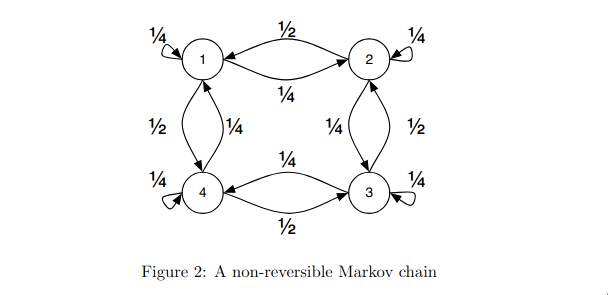
\includegraphics[width=0.8\textwidth]{assets/non_reversible_markov_chain.png}
  \label{fig:non_reversible_markov_chain}
\end{figure}
\begin{note}
  Despite being irreducible and aperiodic the above is not a reversible markov chain. 
\end{note}

\begin{definition}
  A reversible markov chain is defined specifically as: let $P[X_0 = i] = \pi_i$ where $\pi$ is the stationary distribution. Then,
  \[
    P[X_{n-1}=j\mid X_n = i] = \frac{P[X_{n-1}=j , X_n = i]}{P[X_n=i]} = \frac{P[X_n = i \mid  X_{n-1} = i] \cdot P[X_{n-1}=j]}{P[X_n = i]} = \frac{P_{i,j} \cdot \pi_j}{\pi_i} 
  .\] 
  If $\frac{P_{j,i} \pi_j}{\pi_i} = P_{i,j}$. We call the chain reversible.  
\end{definition}

\begin{corollary}
  An irreducible, aperiodic markov chain is reversible if $\pi_i P_{i,j} = \pi_j P_{j,i} \forall i,j \in \Omega$. flow in = flow out at equilibrium.
\end{corollary}


\begin{figure}[h]
  \centering
  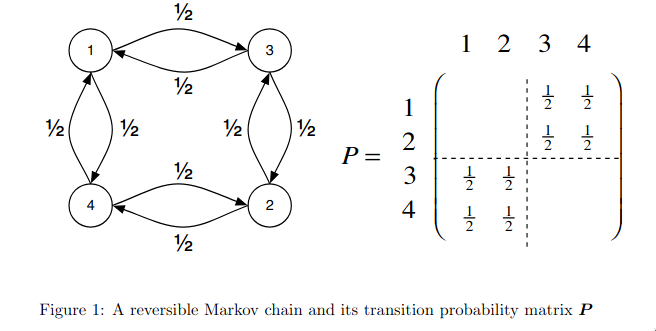
\includegraphics[width=0.8\textwidth]{assets/reversible_markov_chain_ex.png}
  \label{fig:reversible_markov_chain_ex}
\end{figure}

\begin{prop}
  Let $w$ be a row vector such that:
   \[
  w_i P_{i,j} = w_j P_{j,i} \forall i,j \in \Omega
  .\] 
  Then $w = c \pi$  where  $c = \sum_{i=1}^{n} w_i$. and the markov chain is reversible.

  \begin{proof}
    From a previous theorem it suffices to show that $w = wP$. Then,
     \begin{align*}
       (wP)_{k } &= \sum_{j \in \Omega} w_j P_{j,k} \\
                 &= \sum_{j \in \Omega} w_k P_{k,j} \\
                 &= w_k \cdot \left( \sum_{j}  P_{k,j} \right) \\
                 &= w_k
    .\end{align*}
    $w$ is the row eigenvector and a multiple of the stationary distribution! 
  \end{proof}
\end{prop}

\begin{note}
  Thus, we can find if a markov chain is reversible and find its stationary distribution by constructing $w$ through some guess for  $w_i$. The process will fail if the markov chain is not reversible 
\end{note}

\begin{figure}[H]
  \centering
  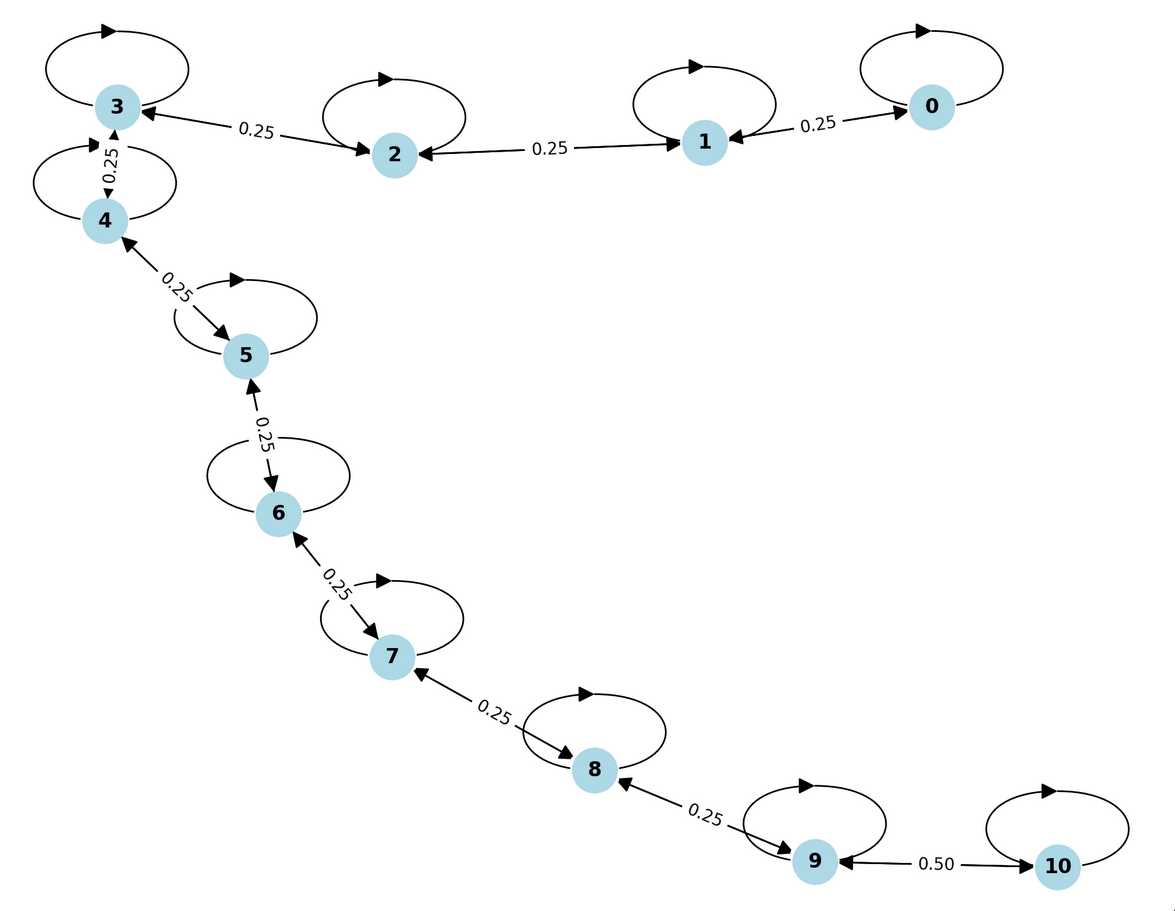
\includegraphics[width=0.8\textwidth]{assets/reversible_markov_chain_ex2.png}
  \caption{Reversible Markov Chain Problem $P_{10}$}
  \label{fig:reversible_markov_chain_ex2}
\end{figure}
We can construct the stationary distribution using $w$ to satisfy $w_j P_{i,j} = w_j P_{j,i}$ . We have a degree of freedom so let's let $w_0 = 1$. Then,
\begin{align*}
  & w_0 \cdot P_{0,1} = w_1 \cdot P_{1,0} \\
  & 1 \cdot \frac{1}{2} = w_1 \cdot \frac{1}{4} \Rightarrow w_1 = 2 \\
  & \ldots P_{0,3} = P_{3,0 } = P_{n,0} = P_{0,n} = 0
.\end{align*}
Then generalizing,
\[
w_1 \frac{1}{4}&=  w_2 \frac{1}{4} \Rightarrow w_2 = 2
.\] 
and so $w_1 = w_2 = \ldots = w_{n-1} = 2$. Then,

\begin{align*}
 w_{n-1} \cdot P_{n,n-1} = w_n P_{n,n-1} \\
 2 \cdot \frac{1}{4} = w_n \frac{1}{2}  \Rightarrow w_n = 1
.\end{align*}

Then, normalizing $w$ to  $\pi$, we get $\pi = \left( \frac{1}{2n}, \frac{1}{n}, \ldots, \frac{1}{n}, \frac{1}{2n} \right) $ is the stationary distribution $P_n$.

\section{Classes of Reversible Markov chains}
\begin{definition}
  Let $G$ a graph on  $n$ vertices  $V = \{1,\ldots,n\} $ and $E=$ undirected pairs of vertices. Given $G$, we define markov chain where if $x_n = v$,  $x_n+1$ is uniformly chosen amongst the neighbors of  $v$ i.e.
   \[
  P_{v,w} = \frac{1}{\text{ edges adjacent to v}} = \frac{1}{\text{deg(v)}} \text{ if } (v,w) \in E
  .\]
\end{definition}

\begin{prop}
  Every random walk on a graph is reversible. 

  \begin{proof}
    Let $w_v = \text{ number of edges incident to $v$ is }$. Then by construction,
    \[
    w_v \cdot P_{v,w} = \begin{cases}
      0, \text{ if  w is not a neighbor of v}\\
      1, \text{ if $(v,w) \in E$} = w_w P_{w,v}
    \end{cases}
    .\] 
    And in particular,
    \[
     \pi_{v} = \frac{w_v}{\sum_{w_v}} = \frac{\text{ number of edges incident to v}}{2 \cdot \text{ simple edges } + \text{ self loops }}
    .\] 
  \end{proof}
\end{prop}

\end{document}
